\documentclass[12pt]{article}
\usepackage[utf8]{inputenc}
\usepackage{amsmath}
\usepackage{amsfonts}
\usepackage{amssymb}
\usepackage{amsthm}
\usepackage{graphicx}
\usepackage[labelformat=simple]{subcaption}
\usepackage{verbatim}
\usepackage[left=2.54cm, right=2.54cm, top=2.54cm, bottom=2.54cm]{geometry}
\usepackage{pgf}
\usepackage{tikz,braids}
\usetikzlibrary{positioning}
\usepackage[export]{adjustbox}
\theoremstyle{definition}
\newtheorem{defi}{Definición}[section]
\newtheorem{teor}{Teorema}[section]
\newtheorem{prop}{Proposición}[section]
\newtheorem{ejem}{Ejemplo}[section]

\renewcommand\thesubfigure{(\alph{subfigure})}



\title{Grupo de trenzas y criptografía}
\author{Fernando de la Hoz Moreno}
\date{}
    

\begin{document}

\maketitle

\section{Generalidades sobre grupos}

\begin{defi}[Grupo]
Un grupo es una estructura algebraica formada por un conjundo $G\neq\emptyset$ y una operación interna $G\times G$ a la que llamaremos \textit{producto}. Esta operación asigna a cada pareja $(x,y)$ el elemento $xy$ y verifica las siguientes propiedades:

\begin{enumerate}
\item Propiedad asociativa: $x(yz) = (xy)z$ $\ \ \forall x,y,z\in G$.
\item Existencia de elemento neutro: Existe $1\in G$ tal que $x1= x = 1x\ \ \forall x\in G$.
\item Existencia de elemento simétrico: Para cada $x \in G$ existe $x^{-1}\in G$.
\end{enumerate}
\end{defi}

\begin{prop}
Sea $G\neq\emptyset$ y el producto $G\times G\rightarrow G$ $(x,y)\rightarrow xy$ verificando

\begin{enumerate}
\item Propiedad asociativa: $x(yz) = (xy)z$ $\ \ \forall x,y,z\in G$.
\item Existencia de elemento neutro: Existe $1\in G$ tal que $x1= x = 1x\ \ \forall x\in G$.
\item Existencia de elemento simétrico: Para cada $x \in G$ existe $x^{-1}\in G$.
\end{enumerate}

\end{prop}

\begin{defi}[Subgrupo]
Sea $G$ un grupo. Un subgrupo de $G$ es un subconjunto $H\subseteq G$, $H\neq\emptyset$ que verifica
\begin{enumerate}
\item $xy\in H\ \ \ \forall x,y\in H$ 
\item $1\in H$
\item $x^{-1}\in H\ \ \ \forall x\in H$
\end{enumerate}

Si $H$ es un subgrupo de $G$, lo denotaremos $H\leq G$.

\end{defi}

\begin{defi}[Subgrupo generado]
Sea G un grupo y $X\subseteq G$ un subconjunto $X\neq\emptyset$. Definimos el subgrupo generado por $X$, que denotaremos $<X>$, como el menor subgrupo de $G$ que contiene al conjunto $X$. Se tiene que

$$<X>\ \ =\bigcap_{X\subset K\in Sub(G)}K$$

\end{defi}

\begin{prop}
Para $X\subseteq G$ siendo $X\neq\emptyset$ se tiene que

$$<X>\  = \{x_1^{n_1}x_2^{n_2}\cdot\cdot\cdot x_r^{n_r} :\ x_i\in X,\ n_i\in\mathbb{Z},\ r\geq 1\}$$

\end{prop}

\begin{prop}
Si $G$ es un grupo finito y $X\subseteq G$ siendo $X\neq\emptyset$, entonces

$$<X>\  = \{x_1^{n_1}x_2^{n_2}\cdot\cdot\cdot x_r^{n_r} :\ x_i\in X,\ n_i\in\mathbb{N},\ r\geq 1\}$$

\end{prop}

Denotaremos al subgrupo generado por un único elemento $a\in G$ por $<a>\ = \{a^n:n\in\mathbb{Z}\}$. Si $G$ es finito entonces $<a> = \{a^n:n\geq 0\}$.

Si $X=\{x_1,x_2,...,x_k\}\subseteq G$ es un subconjunto finito entonces $<x_1,x_2,...,x_k>=<X>$.

Si $<X> = G$ diremos que $X$ es un conjunto de generadores de G. Diremos que $G$ es finitamente generado si existe $\{x_1,x_2,...,x_k\}\subseteq G.$ tal que $<x_1,x_2,...,x_k>=G$. Diremos que el grupo G es ciclico si existe $a\in G$ tal que $<a>=G$




\section{Introducción a las trenzas}

\begin{comment}
\begin{defi}[$n$-trenza]\label{n_trenza}
Sea $\mathbb{D}$ el cubo unidad, de manera que $\mathbb{D} = \{(x,y,z)\ |\ 0\leq x,y,z\leq 1\}$. En la cara superior del cubo se situan $n$ puntos, $A_1, A_2,...,A_n$, y, de igual manera, se situan $n$ puntos en la cara inferior $B_1, B_2,...,B_n$.
\newline
\newline
Por conveniencia, tomaremos los puntos $A_1=(\frac{1}{2}, \frac{1}{n+1},1),\ A_2=(\frac{1}{2}, \frac{2}{n+1},1),\ ...\ ,\ A_n=(\frac{1}{2}, \frac{n}{n+1},1)$ y $B_1=(\frac{1}{2}, \frac{1}{n+1},0),\ B_2=(\frac{1}{2}, \frac{2}{n+1},0),\ ...\ ,\ B_n=(\frac{1}{2}, \frac{n}{n+1},0)$.
\newline
\newline
Ahora unimos los $n$ puntos $A_1,\ A_2,\ \dotsc\ ,A_n$ con $B_1,\ B_2,\ \dotsc\ ,B_n$ por medio de $n$ segmentos poligonales/arcos $d_1,\ d_2,\ \dotsc\ ,d_n$ (estrictamente hablando, los segmentos deberían ser poligonales, pero, con el fin de hacer los diagramas de manera que sean más faciles de ver al dibujarlos, dibujaremos estos arcos como curvas suaves). Sin embargo, los arcos solo pueden unir de forma que cumplan las siguientes tres condiciones:
\begin{enumerate}
\item $d_1,\ d_2,\ \dotsc\ ,d_n$ son mutuamente disjuntos.
\item Cada $d_i$ conecta algún $A_j$ a algún $B_k$, donde $j$ y $k$ podrían ser o no iguales, pero $d_i$ no permite conectar $A_j$ a $A_k$ (o $B_j$ a $B_k$).
\item Cada plano $E_s$ (llamado plano de nivel), tal que z = s y $s\in [0,1]$ (en otras palabras paralelo al plano-xy) interseca a cada arco $d_i$ en un solo punto.
\end{enumerate}
 Tal configuración de de $n$ arcos $d_1,\ \dotsc\ ,d_n$ (con puntos extremos $A_1,\ A_2,\ \dotsc\ ,A_n$ y $B_1,\ B_2,\ \dotsc\ ,B_n$) es llamada una $n$-trenza, o una trenza con $n$ cadenas. Como cabría de esperar, $d_i$ es llamado una (trenza) cadena (o equivalentemente la $i$-ésima (trenza) cadena).
\end{defi}
\ 
\newline
Vamos a denotar al conjunto de todas las $n$-trenzas por $\mathcal{B}_n$. A continuación definimos un solo movimiento, al que denominaremos como \textit{movimiento elemental}.


\begin{defi}[movimiento elemental]\label{mov_elem}
Supongamos que $\mathbb{D}$ es el cubo unidad y que dentro de este cubo hay un número de cadenas como las definidas en la Definición \ref{n_trenza}. (Para el proposito de esta definición, necesitamos restringir y trabajar exclusivamente con la imagen poligonal de una cadena). Sea $\mathit{AB}$ un segmento de la cadena $d$. Sea $\mathit{C}$ un punto en $\mathbb{D}$ tal que el triángulo $\triangle\mathit{ABC}$ (en $\mathbb{D}$) no interseca a ninguna otra cadena y solo se encuentra con $d$ en $\mathit{AB}$. 
\newline
\newline
Si suponemos que $\mathit{AC}\cup\mathit{CB}$ interseca a todos los planos de nivel $E_s$ con $s\in[0,1]$ como mucho en un punto entonces a la operación de reemplazar $AB$ por $\mathit{AC}\cup\mathit{CB}$, a la cual notaremos por $\Omega$, se le denomina \textit{movimiento elemental}. También podemos realizar la operación inversa, sustituyento $\mathit{AC}\cup\mathit{CB}$ por $AB$, a la que notamos por $\Omega^{-1}$.

\end{defi}

\begin{defi}[Equivalencia de trenzas]\label{eq_trenzas}
Decimos que dos $n$-trenzas, $\beta$ y $\beta'$, son equivalentes si se puede transformar $\beta$ en $\beta '$ tras aplicar un número finito de movimientos elementales sobre $\beta$. Denotamos esta equivalencia como $\beta \sim \beta'$.
\end{defi}

\end{comment}

\begin{defi}[Trenza geométrica]\label{trenza_geom}
Una trenza geométrica de $n$ hebras, con $n \geq 1$, es un subconjunto $\mathcal{B}\subset\mathbb{R}^2\times I$ formado por $n$ intervalos topológicos disjuntos llamados hebras de tal manera que la proyección $\mathbb{R}^2\times I\rightarrow I$ establezca un homeomorfismo de cada hebra en $I$ y
$$$$
$$\mathcal{B}\cap(\mathbb{R}^2\times \{0\})=\{(1,0,0),(2,0,0),...,(n,0,0)\}$$
$$\mathcal{B}\cap(\mathbb{R}^2\times \{1\})=\{(1,0,1),(2,0,1),...,(n,0,1)\}$$
$$$$
Cada hebra de $\mathcal{B}$ interseca con el plano $\mathbb{R}^2\times \{t\}$ con $t\in I$ en un único punto y conecta un punto $(i,0,0)$ con un punto $(s(i),0,0)$ donde $i,s(i)\in\{1,2,...,n\}$. La sucesión $(s(1),s(2),...,s(n))$ es una permutación del conjunto $\{1,2,...,n\}$ llamada permutación subyacente de $\mathcal{B}$
\end{defi}


Decimos que dos trenzas geométricas $\mathcal{B}$ y $\mathcal{B}'$ son isotópicas si podemos deformar de manera continua $\mathcal{B}$ en $\mathcal{B}'$. Más formalmente, $\mathcal{B}$ y $\mathcal{B}'$ son isotópicas si existe una función continua $F : \mathcal{B} \times I \rightarrow \mathbb{R}^2\times I$ de tal manera que para cada $s\in I$, la función $F_s : \mathcal{B}\rightarrow \mathbb{R}^2\times I$ con $F_s(x)= F(x,s)$ es un embebimiento cuya imagen es una trenza geométrica de $n$ hebras, cumpliendo que $F_0 = id_{\mathcal{B}}: \mathcal{B}\rightarrow \mathcal{B}$ y $F_1(\mathcal{B}) = \mathcal{B}'$. Debido a que la imagen de $F_s$ es una trenza geométrica y $F$ es una función continua tenemos automáticamente que la imagen del punto final de cada hebra por $F_s$ es el mismo.
\newline
\newline
Tanto la función $F$ como la familia de hebras geométricas $\{F_s(\mathcal{B})\}_{s\in I}$ se llaman \textit{isotopía} de $\mathcal{B}$ en $\mathcal{B}'$. Se ve facilmente que la relación de isotopía es una relación de equivalencia. Al conjunto de clases de equivalencia correspondientes se les denomina \textit{trenzas de n hebras} y lo denotamos por $\mathcal{B}_n$
\newline
\newline
Para poder especificar una trenza geométrica se puede utilizar la proyección en $\mathbb{R}\times\{0\}\times I$ e indicar de alguna manera que hebra esta por encima de otra cuando se crucen. Solo se podrá aplicar esta solución en trenzas geométricas cuya proyección solo tenga puntos donde se crucen a lo más dos hebras. Pasamos a definir formalmente un diagrama de trenza.


\begin{defi}[Diagrama de trenza]\label{diagrama_trenza}
Un díagrama de trenzas de $n$ hebras es un conjunto $\mathcal{D}\subset\mathbb{R}\times I$ formado por la unión de $n$ intervalos topológicos llamados hebras y que cumplen las siguientes condiciones: 
\begin{enumerate}
\item La proyección de $\mathbb{R}\times I\rightarrow I$ es un homeomorfismo.
\item Cada punto de $\{1,2,...,n\}\times\{0,1\}$ es un punto final de la hebra.
\item Cada punto de $\mathbb{R}\times I$ pertenece como mucho a dos hebras. En cada punto donde se intersequen dos hebras, estas se cruzaran transversalmente.


\end{enumerate}
\end{defi}

La transversalidad de los cruces y la compacidad de las hebras nos asegura que el número de cruces es finito. Gráficamente la hebra que pasa por debajo en un cruce se representará con una discontinuidad y la que pasa por encima con una linea continua. Cada trenza puede ser representada por un diagrama de trenza y cada diagrama tiene asociada una trenza. Dado $\mathcal{D}$ un diagrama, denotaremos como $\beta(\mathcal{D})$ a la trenza de $n$ hebras asociada.
\newline
\newline
Dos diagramas de trenzas $\mathcal{D}, \mathcal{D}'$ de $n$ hebras se dicen que son isotópicos si se puede establecer una función continua entre $F:\mathcal{D}\times I\rightarrow\mathbb{R}\times I$ tal que para cada $s\in I$ el conjunto $\mathcal{D}_s = F(\mathcal{D}\times s)\subset\mathbb{R\times I}$ es un diagrama de $n$ hebras, con $\mathcal{D}_0 = \mathcal{D}$ y $\mathcal{D}_1 = \mathcal{D}'$. Se entiende que $F$ mapea los cruces de $\mathcal{D}$ en los cruces de $\mathcal{D}_s$ para todo $s\in I$ preservando si los cruces son por debajo o por encima. A la familia de diagramas $\{\mathcal{D}_s\}_{s\in I}$ se le llama \textit{isotopía} de $\mathcal{D}_0 = \mathcal{D}$ en $\mathcal{D}_1 = \mathcal{D}'$.




\begin{figure}[h!]
\centering
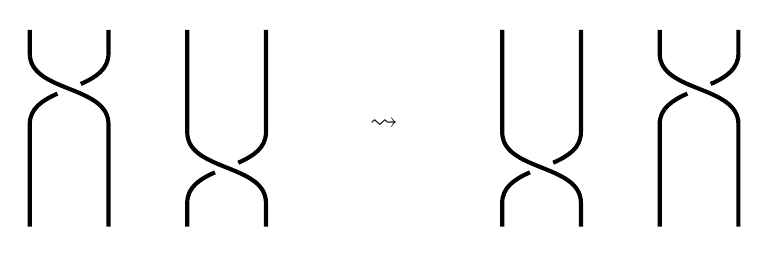
\begin{tikzpicture}
\braid[line width =1.5pt, number of strands = 4, name = b1] (b1) at (-3,0) a_1 a_3;
		\braid[line width =1.5pt, number of strands = 4, name = b1] (b1) at (3,0) a_3 a_1;
		\node[] at (1.5,-1.2){$\leadsto$};
\end{tikzpicture}
\caption{Diagramas isótopicos}
\end{figure}







\begin{defi}[Movimientos de Reidemeister]  Los movimientos de Reidemester  son movimientos locales (afectan a la posición de las hebras dentro de un disco en 
$ \mathbb{R}\times I $ ) en un diagrama de trenzas. Estos estan formados por $\Omega_2$, $\Omega_3$ (Figura \ref{MR}) y sus transformaciones inversas
$\Omega_2^{-1}$, $\Omega_3^{-1}$. 

\end{defi}

\begin{figure}[h!]
\centering
\begin{subfigure}[b]{0.6\linewidth}
\begin{center}
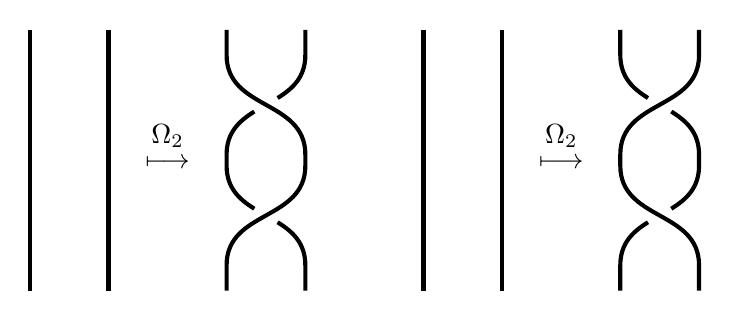
\begin{tikzpicture}
\braid[line width =1.5pt, number of strands = 2, name = b1, height = 80pt] (b1) at (-7,0) a1;
\braid[line width =1.5pt, number of strands = 2, name = b1, height = 40pt] (b1) at (-4.5,0) a_1 a_1^{-1};

		\node[] at (-5.25,-1.7){$\longmapsto$};
		\node[] at (-5.25,-1.35){$\Omega_2$};

\braid[line width =1.5pt, number of strands = 2, name = b1, height = 80pt] (b1) at (-2,0) a1;
\braid[line width =1.5pt, number of strands = 2, name = b1, height = 40pt] (b1) at (0.5,0) a_1^{-1} a_1;

		\node[] at (-0.25,-1.7){$\longmapsto$};
		\node[] at (-0.25,-1.35){$\Omega_2$};
\end{tikzpicture}

\caption{}
\end{center}
\end{subfigure} 


\begin{subfigure}[b]{0.6\linewidth}
\begin{center}
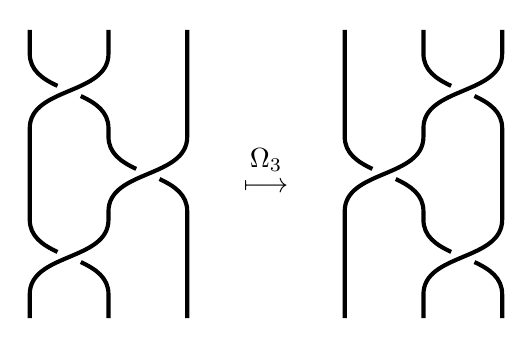
\begin{tikzpicture}
\braid[line width =1.5pt, number of strands = 3, name = b1, height = 30pt] (b1) at (-8.25,0) a_1^{-1}  a_2^{-1} a_1^{-1};
\braid[line width =1.5pt, number of strands = 3, name = b1, height = 30pt] (b1) at (-4.25,0) a_2^{-1} a_1^{-1} a_2^{-1};

		\node[] at (-5.25,-2.0){$\longmapsto$};
		\node[] at (-5.25,-1.65){$\Omega_3$};


\end{tikzpicture}

\caption{}
\end{center}
\end{subfigure} 


\caption{Movimientos de Reidemeister}
\label{MR}
\end{figure}


Estos movimientos preservan la correspondencia entre diagrama de trenza y trenza. Decimos que dos diagramas de trenzas $\mathcal{D}, \mathcal{D}'$ son $\mathcal{R}$\textit{-equivalentes} si $\mathcal{D}$ puede ser transformado en $\mathcal{D}'$ mediante una sucesión finita de isotopías y movimientos de Reidemeister. Esta claro que si $\mathcal{D}, \mathcal{D}'$ son $\mathcal{R}$\textit{-equivalentes}, entonces $\beta(\mathcal{D}) = \beta(\mathcal{D'})$.
\newline

Hemos construido dos equivalencias, una para trenzas geométricas y otra para diagramas de trenzas. El Teorema \ref{teor:equiv} nos permite trabajar indiferentemente con unas o con otras utilizando ambas equivalencias.


\begin{teor}
Dos diagramas de trenzas representan trenzas geométricas isotópicas si y solo si son $\mathcal{R}$\textit{-equivalentes}.
\label{teor:equiv}
\end{teor}
\section{Grupo de trenzas}
\begin{defi}[Producto de hebras]
Dado dos diagrama de trenzas $\mathcal{D}_1$, $\mathcal{D}_2$, representando las trenzas de $n$ hebras $\beta_1$ y $\beta_2$ respectivamente, definimos el producto de diagramas $\mathcal{D}_1\mathcal{D}_2$ concatenando $\mathcal{D}_1$ en la parte superior de $\mathcal{D}_2$ y reduciendo el diagrama resultante en $\mathbb{R}\times I$. Entonces el producto de trenzas $\beta_1\beta_2$ es la trenza  asociada al diagrama producto $\mathcal{D}_1\mathcal{D}_2$.

\end{defi} 

\begin{ejem}
Sean $\beta_1,\beta_2\in \mathcal{B}_3$, cuyos diagramas se pueden ver en \subref{subfig:factores}, el resultado del producto $\beta_1\beta_2$ 
\begin{figure}[h!]
\centering
	\begin{subfigure}[b]{0.45\linewidth}
		\begin{center}
		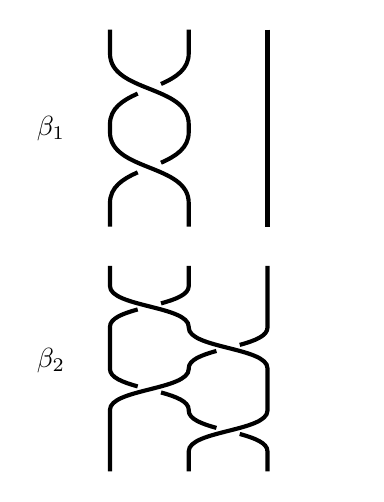
\begin{tikzpicture}
		\braid[line width =1.5pt, number of strands = 3, name = b1] (b1) at (-3,3) a_1 a_1;
	\node[] at (-3.75,1.75){$\beta_1$};
	\node[] at (0,0){};
		\braid[line width =1.5pt, height = 15pt, nudge factor = 0.01, control factor = 0.5, name = b2] (b2) at (-3,0) a_1 a_2 a_1^{-1} a_2^{-1};
		\node[] at (-3.75,-1.2){$\beta_2$};

		\end{tikzpicture}
		\end{center}
		
		\caption{}
		\label{subfig:factores}
	\end{subfigure}
	\begin{subfigure}[b]{0.45\linewidth}
		\begin{center}
		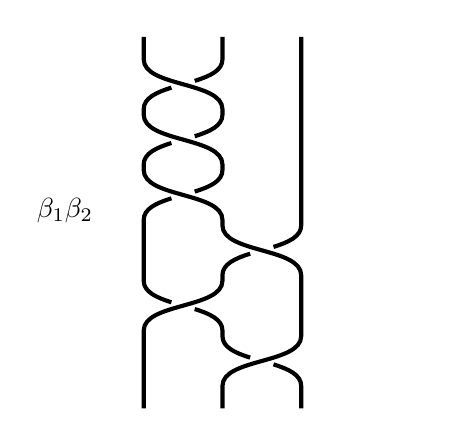
\begin{tikzpicture}
		\braid[line width =1.5pt, height = 20pt, number of strands = 3]  a_1 a_1 a_1 a_2 a_1^{-1} a_2^{-1};
		\node[] at (0,-2.2){$\beta_1\beta_2$};
	\node[] at (4.5,0){};
		\end{tikzpicture}
		\end{center}
		\caption{}
	\end{subfigure}
	\caption{Producto de dos hebras}
	\label{fig:producto_hebras}
\end{figure}
\end{ejem}








\textit{Nota: Formalmente la longitud de los diagramas debería ser constante, pero para una mejor visualización de estos no se ha tenido en cuenta.}
\newline
\newline
De forma clara se ve que el elemento neutro para el producto de trenzas, por ambos lados, es la trenza con el diagrama cuyas hebras se encuentran paralelas entre sí (Figura \ref{fig:elem_neu}).
\begin{comment}
hola
\end{comment}

\begin{figure}[h!]
\begin{center}
		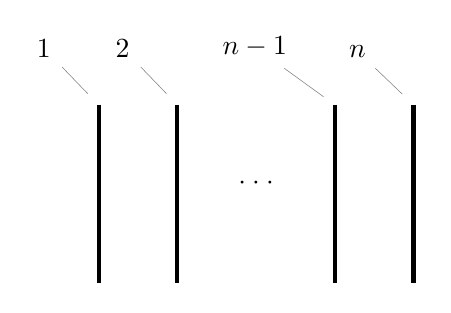
\begin{tikzpicture}
		\braid[line width =1.5pt, height = 50pt, number of strands = 2, name = a]  a1;
		\node[at=(a-1-s),pin=north west:1]  {};
		\node[at=(a-2-s),pin=north west:2]  {};
		\node[] at (3,-1){$\cdot\cdot\cdot$};
		\braid[line width =1.5pt, height = 50pt, number of strands = 2, name = b] at (4,0) a1;
		\node[at=(b-1-s),pin=north west:$n-1$]  {};
		\node[at=(b-2-s),pin=north west:$n$]  {};
		\end{tikzpicture}
		\end{center}
		\caption{Elemento neutro}
		\label{fig:elem_neu}
\end{figure}


Trivialmente también se tiene la asociatividad del producto de trenzas como se puede ver en la .

\begin{ejem}[Asociatibidad]





\begin{figure}[h!]
\centering
	\begin{subfigure}[b]{0.8\linewidth}
		\begin{center}
		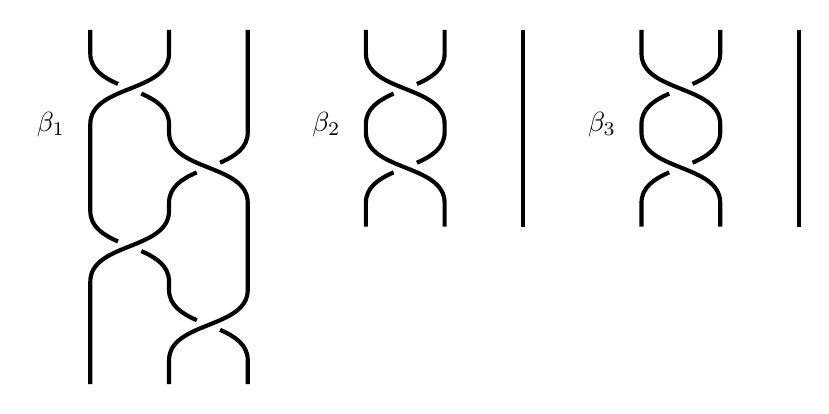
\begin{tikzpicture}
		\braid[line width =1.5pt, number of strands = 3] (b1) at (-4,0) a_1 a_1;
		\braid[line width =1.5pt, number of strands = 3] (b1) at (-7.5,0) a_1^{-1} a_2 a_1^{-1} a_2^{-1};
		\braid[line width =1.5pt, number of strands = 3] (b1) at (-0.5,0) a_1 a_1;
	\node[] at (-4.5,-1.2){$\beta_2$};
	\node[] at (-8,-1.2){$\beta_1$};
	\node[] at (-1,-1.2){$\beta_3$};

		\end{tikzpicture}
		\end{center}
		
		\caption{}
		\label{subfig:factores}
	\end{subfigure}
	
	\begin{subfigure}[b]{0.45\linewidth}
		\begin{center}
		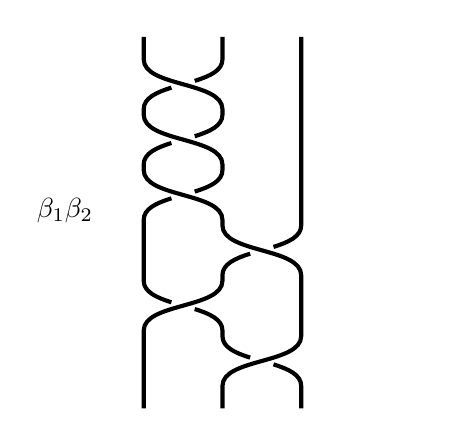
\begin{tikzpicture}
		\braid[line width =1.5pt, height = 20pt, number of strands = 3]  a_1 a_1 a_1 a_2 a_1^{-1} a_2^{-1};
		\node[] at (0,-2.2){$\beta_1\beta_2$};
	\node[] at (4.5,0){};
		\end{tikzpicture}
		\end{center}
		\caption{}
	\end{subfigure}
	\begin{subfigure}[b]{0.45\linewidth}
		\begin{center}
		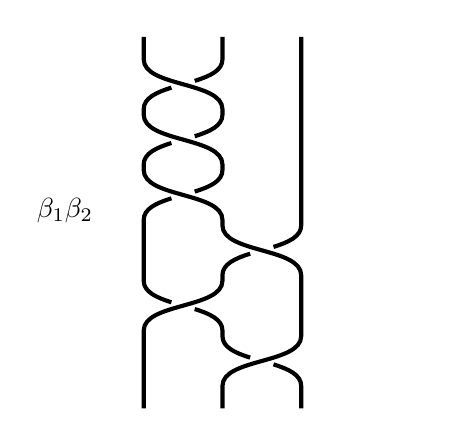
\begin{tikzpicture}
		\braid[line width =1.5pt, height = 20pt, number of strands = 3]  a_1 a_1 a_1 a_2 a_1^{-1} a_2^{-1};
		\node[] at (0,-2.2){$\beta_1\beta_2$};
	\node[] at (4.5,0){};
		\end{tikzpicture}
		\end{center}
		\caption{}
	\end{subfigure}
	\caption{Producto de dos hebras}
	\label{fig:producto_hebras}
\end{figure}



\end{ejem}




		

\end{document}

